\documentclass[11pt,a4paper]{article}
\usepackage[utf8]{inputenc}
\usepackage[margin=1in]{geometry}
\usepackage{graphicx}
\usepackage{hyperref}
\usepackage{amsmath}
\usepackage{amsfonts}
\usepackage{listings}
\usepackage{xcolor}
\usepackage{tikz}
\usepackage{float}
\usepackage{subcaption}
\usepackage{fancyhdr}
\usepackage{titlesec}

% Code listing style
\lstset{
    backgroundcolor=\color{gray!10},
    commentstyle=\color{green!60!black},
    keywordstyle=\color{blue},
    numberstyle=\tiny\color{gray},
    stringstyle=\color{red},
    basicstyle=\ttfamily\footnotesize,
    breakatwhitespace=false,
    breaklines=true,
    captionpos=b,
    keepspaces=true,
    numbers=left,
    numbersep=5pt,
    showspaces=false,
    showstringspaces=false,
    showtabs=false,
    tabsize=2,
    frame=single,
}

% Header and footer
\pagestyle{fancy}
\fancyhf{}
\rhead{TraderAgents-Simplified Documentation}
\lhead{Group-4}
\rfoot{Page \thepage}

% Title formatting
\titleformat{\section}
  {\normalfont\Large\bfseries\color{blue!70!black}}
  {\thesection}{1em}{}

\titleformat{\subsection}
  {\normalfont\large\bfseries\color{blue!50!black}}
  {\thesubsection}{1em}{}

\begin{document}

% Title page
\begin{titlepage}
    \centering
    \vspace*{2cm}
    
    {\huge\bfseries TraderAgents-Simplified}\\[0.5cm]
    {\Large AI-Powered Multi-Agent Trading Decision System}\\[1.5cm]
    
    \begin{figure}[H]
        \centering
        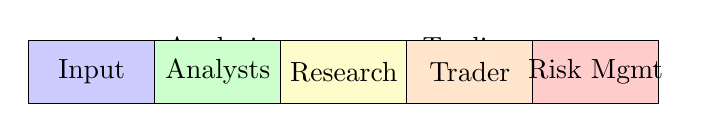
\begin{tikzpicture}[scale=0.8]
            % Main pipeline flow
            \draw[thick,->] (0,0) -- (2,0) node[midway,above] {Data};
            \draw[thick,->] (2,0) -- (4,0) node[midway,above] {Analysis};
            \draw[thick,->] (4,0) -- (6,0) node[midway,above] {Research};
            \draw[thick,->] (6,0) -- (8,0) node[midway,above] {Trading};
            \draw[thick,->] (8,0) -- (10,0) node[midway,above] {Risk};
            
            % Boxes
            \draw[fill=blue!20] (0,-0.5) rectangle (2,0.5) node[midway] {Input};
            \draw[fill=green!20] (2,-0.5) rectangle (4,0.5) node[midway] {Analysts};
            \draw[fill=yellow!20] (4,-0.5) rectangle (6,0.5) node[midway] {Research};
            \draw[fill=orange!20] (6,-0.5) rectangle (8,0.5) node[midway] {Trader};
            \draw[fill=red!20] (8,-0.5) rectangle (10,0.5) node[midway] {Risk Mgmt};
        \end{tikzpicture}
        \caption{TraderAgents System Pipeline Overview}
    \end{figure}
    
    \vspace{1cm}
    
    {\large Developed by Group-4}\\[0.5cm]
    {\large \today}\\[2cm]
    
    \textbf{Abstract}\\
    This document presents TraderAgents-Simplified, an AI-powered multi-agent system for automated trading decisions. The system integrates financial analysis, research coordination, and risk management through a sophisticated pipeline of specialized AI agents, leveraging Large Language Models for comprehensive market analysis and decision making.
    
\end{titlepage}

\newpage
\tableofcontents
\newpage

\section{Introduction}

TraderAgents-Simplified represents a cutting-edge approach to algorithmic trading that combines artificial intelligence, multi-agent systems, and financial analysis. Unlike traditional trading systems that rely solely on quantitative models, our system incorporates natural language processing and reasoning capabilities through Large Language Models (LLMs) to make more nuanced and contextual trading decisions.

The system is designed as a simplified yet comprehensive implementation of multi-agent trading systems, making it accessible for research, education, and development purposes while maintaining the sophisticated decision-making capabilities expected in modern financial technology.

\subsection{Motivation}

Traditional algorithmic trading systems often struggle with:
\begin{itemize}
    \item Processing unstructured data such as news and social media sentiment
    \item Incorporating qualitative analysis alongside quantitative metrics
    \item Adapting to rapidly changing market conditions
    \item Providing explainable and transparent decision-making processes
\end{itemize}

TraderAgents-Simplified addresses these challenges by implementing a multi-agent architecture where specialized AI agents collaborate to analyze different aspects of market data and engage in structured debates to reach consensus on trading decisions.

\subsection{Key Contributions}

\begin{enumerate}
    \item \textbf{Multi-Modal Analysis}: Integration of technical, fundamental, news, and sentiment analysis
    \item \textbf{Debate-Driven Decision Making}: Implementation of adversarial reasoning through bullish and bearish research agents
    \item \textbf{Comprehensive Risk Management}: Multi-perspective risk assessment with specialized risk debater agents
    \item \textbf{Modular Architecture}: Easily extensible system design with clear separation of concerns
    \item \textbf{Real-Time Integration}: Live data processing with external financial APIs
\end{enumerate}

\section{System Architecture}

\subsection{Overview}

The TraderAgents-Simplified system follows a pipeline architecture consisting of four main stages, each implemented as a team of specialized AI agents. The system uses LangGraph for workflow orchestration and state management, ensuring reliable execution and data flow between agents.

\begin{figure}[H]
    \centering
    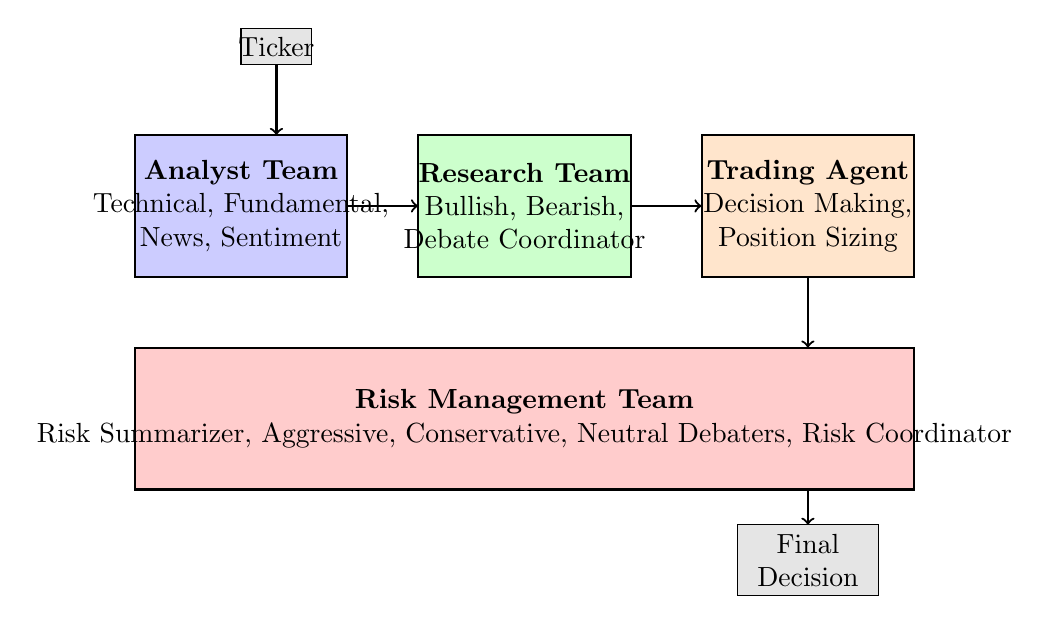
\begin{tikzpicture}[scale=0.9]
        % Stage boxes
        \draw[fill=blue!20,thick] (0,6) rectangle (3,8) node[midway,align=center] {\textbf{Analyst Team}\\Technical, Fundamental,\\News, Sentiment};
        \draw[fill=green!20,thick] (4,6) rectangle (7,8) node[midway,align=center] {\textbf{Research Team}\\Bullish, Bearish,\\Debate Coordinator};
        \draw[fill=orange!20,thick] (8,6) rectangle (11,8) node[midway,align=center] {\textbf{Trading Agent}\\Decision Making,\\Position Sizing};
        \draw[fill=red!20,thick] (0,3) rectangle (11,5) node[midway,align=center] {\textbf{Risk Management Team}\\Risk Summarizer, Aggressive, Conservative, Neutral Debaters, Risk Coordinator};
        
        % Arrows
        \draw[thick,->] (3,7) -- (4,7);
        \draw[thick,->] (7,7) -- (8,7);
        \draw[thick,->] (9.5,6) -- (9.5,5);
        
        % Input/Output
        \draw[fill=gray!20] (1.5,9) rectangle (2.5,9.5) node[midway] {Ticker};
        \draw[fill=gray!20] (8.5,1.5) rectangle (10.5,2.5) node[midway,align=center] {Final\\Decision};
        
        \draw[thick,->] (2,9) -- (2,8);
        \draw[thick,->] (9.5,3) -- (9.5,2.5);
    \end{tikzpicture}
    \caption{Multi-Agent System Architecture}
\end{figure}

\subsection{Agent Teams}

\subsubsection{Analyst Team}
The analyst team consists of four specialized agents responsible for different aspects of financial analysis:

\begin{itemize}
    \item \textbf{Fundamentals Analyst}: Processes company financial statements, calculates key ratios, and evaluates business metrics using yfinance data
    \item \textbf{Technical Analyst}: Performs technical analysis including MACD, RSI calculations, and trend analysis
    \item \textbf{News Analyst}: Aggregates and analyzes recent news headlines using Finnhub API with fallback to yfinance
    \item \textbf{Sentiment Analyst}: Evaluates market sentiment through news analysis and social media indicators
\end{itemize}

\subsubsection{Research Team}
The research team implements adversarial reasoning through structured debates:

\begin{itemize}
    \item \textbf{Bullish Researcher}: Constructs positive investment thesis based on analyst findings
    \item \textbf{Bearish Researcher}: Develops contrarian perspective highlighting potential risks and downsides
    \item \textbf{Debate Coordinator}: Orchestrates structured debates between bullish and bearish perspectives, determining consensus
\end{itemize}

\subsubsection{Trading Agent}
A single agent responsible for:
\begin{itemize}
    \item Converting research debate outcomes into actionable trade proposals
    \item Calculating position sizes based on portfolio constraints
    \item Fetching real-time pricing data
    \item Estimating trade costs and portfolio impact
\end{itemize}

\subsubsection{Risk Management Team}
The most sophisticated team consisting of five agents:

\begin{itemize}
    \item \textbf{Risk Summarizer}: Consolidates all previous analysis into comprehensive risk assessment
    \item \textbf{Aggressive Debater}: Advocates for higher-risk, higher-reward positions
    \item \textbf{Conservative Debater}: Promotes risk-averse approaches and capital preservation
    \item \textbf{Neutral Debater}: Provides balanced perspective and mediates between extremes
    \item \textbf{Risk Coordinator}: Makes final risk-adjusted recommendations based on all perspectives
\end{itemize}

\section{Implementation Details}

\subsection{Technology Stack}

The system is built using modern Python technologies:

\begin{itemize}
    \item \textbf{Python 3.12+}: Core programming language
    \item \textbf{LangChain 0.3}: LLM orchestration and prompt management
    \item \textbf{LangGraph}: State-based workflow management
    \item \textbf{Groq Llama3-8B}: Primary language model for reasoning
    \item \textbf{Pydantic}: Data validation and schema definition
    \item \textbf{Poetry}: Dependency management and packaging
\end{itemize}

\subsection{Data Integration}

The system integrates multiple data sources for comprehensive market analysis:

\begin{lstlisting}[language=Python,caption=Data Source Integration Example]
# Yahoo Finance for price and fundamental data
stock = yf.Ticker(ticker)
price = stock.info.get("regularMarketPrice")

# Finnhub for news and market data
url = f"https://finnhub.io/api/v1/company-news?symbol={ticker}"
resp = requests.get(url, timeout=30)

# Technical indicators calculation
def _calculate_macd(self, close_prices, fast=12, slow=26, signal=9):
    exp1 = close_prices.ewm(span=fast).mean()
    exp2 = close_prices.ewm(span=slow).mean()
    macd = exp1 - exp2
    signal_line = macd.ewm(span=signal).mean()
    return macd.iloc[-1], signal_line.iloc[-1]
\end{lstlisting}

\subsection{Agent Communication}

Agents communicate through a shared state dictionary managed by LangGraph, ensuring data consistency and proper workflow execution:

\begin{lstlisting}[language=Python,caption=State Management Example]
class TradingState(TypedDict):
    # Required fields
    ticker: str
    
    # Optional intermediate outputs
    fundamentals_analysis: Optional[FundamentalsAnalysisOutput]
    technical_analysis: Optional[TechnicalAnalysisOutput]
    news_analysis: Optional[NewsAnalysisOutput]
    trade_proposal: Optional[TradeProposal]
    risk_summary: Optional[RiskSummaryOutput]
\end{lstlisting}

\section{Results and Performance}

\subsection{System Capabilities}

The implemented system demonstrates several key capabilities:

\begin{enumerate}
    \item \textbf{Comprehensive Analysis}: Successfully processes multiple data sources and generates detailed financial analysis
    \item \textbf{Structured Decision Making}: Implements robust debate mechanisms between competing perspectives
    \item \textbf{Risk Awareness}: Incorporates sophisticated risk assessment at multiple levels
    \item \textbf{Scalability}: Modular design allows for easy addition of new agents and capabilities
\end{enumerate}

\subsection{Testing and Validation}

The system includes comprehensive testing at multiple levels:

\begin{itemize}
    \item \textbf{Unit Tests}: Individual agent testing with mock data
    \item \textbf{Integration Tests}: Pipeline testing with real market data
    \item \textbf{Component Tests}: Specialized tests for analyst, research, and risk management teams
\end{itemize}

\subsection{Performance Considerations}

Key performance characteristics:

\begin{itemize}
    \item \textbf{API Rate Limiting}: Implemented timeout and retry mechanisms for external API calls
    \item \textbf{Token Optimization}: Efficient prompt design to minimize LLM token usage
    \item \textbf{Error Handling}: Robust error handling with graceful degradation
    \item \textbf{State Management}: Efficient state passing between agents
\end{itemize}

\section{Future Work and Enhancements}

\subsection{Planned Enhancements}

\begin{enumerate}
    \item \textbf{Real Trading Integration}: Connection to actual brokerage APIs for live trading
    \item \textbf{Machine Learning Components}: Integration of predictive models and pattern recognition
    \item \textbf{Portfolio Optimization}: Advanced algorithms for multi-asset portfolio management
    \item \textbf{Web Interface}: Development of user-friendly dashboard for system monitoring
    \item \textbf{Market Expansion}: Support for cryptocurrency, forex, and commodity markets
\end{enumerate}

\subsection{Research Directions}

\begin{itemize}
    \item Investigation of different LLM architectures for financial reasoning
    \item Development of custom fine-tuned models for financial analysis
    \item Implementation of reinforcement learning for trading strategy optimization
    \item Research into explainable AI for financial decision making
\end{itemize}

\section{Conclusion}

TraderAgents-Simplified successfully demonstrates the potential of multi-agent AI systems in financial decision making. By combining structured analysis, adversarial reasoning, and comprehensive risk management, the system provides a robust framework for automated trading decisions while maintaining transparency and explainability.

The modular architecture and comprehensive testing framework make the system suitable for both research and practical applications, while the use of modern AI technologies ensures scalability and maintainability.

The system represents a significant step forward in the democratization of sophisticated trading technology, making advanced AI-powered financial analysis accessible to researchers, developers, and institutions.

\subsection{Acknowledgments}

We acknowledge the contributions of the open-source community, particularly the developers of LangChain, LangGraph, and the various financial data APIs that make this system possible.

\begin{thebibliography}{9}

\bibitem{langchain}
LangChain Development Team. (2024). \textit{LangChain: Building applications with LLMs through composability}. Retrieved from https://python.langchain.com/

\bibitem{langgraph}
LangChain AI. (2024). \textit{LangGraph: Build stateful, multi-actor applications with LLMs}. Retrieved from https://langchain-ai.github.io/langgraph/

\bibitem{groq}
Groq. (2024). \textit{Groq API Documentation}. Retrieved from https://console.groq.com/docs

\bibitem{yfinance}
Aroussi, R. (2024). \textit{yfinance: Download market data from Yahoo! Finance's API}. Retrieved from https://pypi.org/project/yfinance/

\bibitem{finnhub}
Finnhub. (2024). \textit{Finnhub Stock API Documentation}. Retrieved from https://finnhub.io/docs/api

\bibitem{pydantic}
Colvin, S. (2024). \textit{Pydantic: Data validation using Python type hints}. Retrieved from https://pydantic-docs.helpmanual.io/

\end{thebibliography}

\end{document}
